\documentclass{article}
\usepackage[utf8]{inputenc}
\usepackage[french]{babel}
\usepackage{fullpage}
\usepackage{graphicx}
\usepackage{color}
\usepackage{titlesec}
\setlength{\parindent}{1cm}

\title{LSINF1252 - Projet 2 : Factorisation de nombre}
\author{}
\date{May 2015}
\linespread{1.3}

\begin{document}

\begin{titlepage}

\begin{center}
\textsc{\LARGE  Université Catholique de Louvain-la-Neuve}\\[0.5cm]

\textsc{\large Ecole Polytechnique de Louvain\\ 
LSINF1252 - Systèmes informatiques}\\[1cm]

\textsc{\Large   \\  \vspace{0.8cm}- \today -}\\[0.5cm]

\vspace{0.5cm}

{ \huge \bfseries Projet 2 \\
 [0.4cm]}
 
{\Large \textit{Factorisation de nombres}}

\vspace{1.5cm}

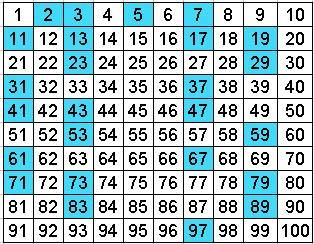
\includegraphics[scale=0.8]{img/couv.jpg}
 
\vspace{1.5cm}
 
\textsc {Monnoyer de Galland de Carnières} Charles\\
\textsc {Paris} Antoine

\end{center}
\end{titlepage}

\section{Introduction}
Dans le cadre de notre cursus en Sciences de l'Ingénieur à l'EPL, orientation Informatique, 
il nous est demandé de venir en aide à un mathématicien devant factoriser des nombres. 
Ce dernier doit déterminer parmi une liste d'entiers non-signés de 64 bits le seul facteur
premier (les facteurs premiers sont des entiers non-signés de 32 bits) qui apparaît une 
et une seule fois.\\

\hspace{1cm}Notre tâche consiste à élaborer un programme pouvant réaliser cela en profitant
 des possibilités d'un ordinateur multiprocesseurs : on utilisera des threads pour accélerer
 la recherche. De plus, le programme devra être en mesure de traiter plusieurs fichiers en
 même temps, pouvant provenir de l'entrée standard, du système de fichiers local ou des serveurs
 Internet, et d'identifier de quel fichier provient le facteur recherché. Enfin, une analyse de
 performances sera réalisée : le programme calculera le temps de son exécution à chaque utilisation.\\

\hspace{1cm}Les nombres passés en arguments de notre programme seront écrits suivant la représentation
\emph{Big Endian}. L'utilisateur pourra faire varier une option \emph{-maxthreads n} correspondant
au nombre maximum de threads de calculs du programme.

\hspace{1cm}Au final, notre programme retournera le facteur premier recherché, le fichier d'origine
 de ce facteur, ainsi que le temps pris par le programme lors de son exécution.

\section{Algorithme de factorisation}
L'élaboration de notre programme a d'abord exigé que nous 
trouvions un algorithme nous permettant de décomposer un nombre en ses facteurs premiers. Nous
 avons donc cherché les divers algorithmes existants et avons finalement retenu la méthode 
triale pour diverses raisons qui seront explicitées par la suite.

\\
\hspace{1cm}Nous avions d'avord envisagé d'employer un algorithme plus élaboré et performant.
 Cependant, il s'est avéré laborieux à mettre en place pour des nombres de 64 bits. De plus,
 les trop bonnes performances dudit algorithme ne permettaient pas d'observer clairement 
l'évolution des performances avec la variation du nombre de threads (notamment car les autres
 étapes indépendantes du nombre de threads ne retrouvaient à consommer beaucoup plus de temps
 que celles dépendantes, obstruant cette analyse). Nous avons donc opté pour la méthode triale.
\\

L'algorithme trial est des plus simples : il s'agit de tester chaque diviseur possible, en commençant
par 2 jusqu'à une valeur déterminée. Si le modulo du nombre et du diviseur potentiel est 0, alors 
le nombre n'est pas premier ; le diviseur est retenu comme facteur premier et le procédé est réitéré
sur la division du nombre par le facteur. Remarquons que le facteur retenu est nécessairement premier,
si ce n'était pas le cas, un diviseur de ce facteur aurait été intercépté avant.\\

Définir la borne d'arrêt des diviseurs potentiels n'est pas compliqué : un nombre ne sera jamais 
divisible par un nombre plus grand que sa racine carrée (excepté lui-même) ; dès lors, il suffit
d'arrêter les tests à sa racine. Si cette borne est atteinte, le nombre est premier.

\section{Architecture générale}
La logique que nous avons suivie pour réaliser notre programme est celle représentée sur la figure \ref{fig:arch}. \\
Premièrement, nous créons autant de threads que de fichiers à traiter : ce sont les \emph{extractors}. 
Leur rôle est d'extraire les nombres un par un des fichiers, de les traduire du \emph{Big Endian}, et de les
mettre dans un premier buffer (\emph{buffer1}). La taille de ce dernier est fixée par le nombre de threads 
\emph{maxthreads n} : en effet, si le buffer est plus petit, les threads ne seront jamais utilisés de façon
optimale, si il est plus grand, les threads n'auront pas vraiment de meilleurs performances et le buffer ne
sera jamais rempli complètement. \\
Ensuite, les threads \emph{factorizer} (dont le nombre est, pour rappel, fixé par la variable \emph{maxthreads n}) se chargent d'extirper les nombres du buffer1 et de les décomposer en facteurs premiers. Pour ce faire, ils cherchent le plus petit diviseur premier du nombre et le mettent dans un second buffer de la même taille que le premier (\emph{buffer2}). Ils réitèrent l'opération sur le quotient du nombre et du diviseur jusqu'à avoir entièrement décomposé le nombre (voir la section précédente pour plus de précisions sur l'algorithme de factorisation).\\
Enfin, un thread unique \emph{save\_data} se charge de prendre les facteurs premiers du second buffer et de les insérer dans la structure chainée \emph{list} en mettant à jour la structure représentant un nombre afin de, au final, pouvoir identifier le facteur premier qui n'apparait qu'une seule fois.\\

\begin{figure}[ht]
	\centering
	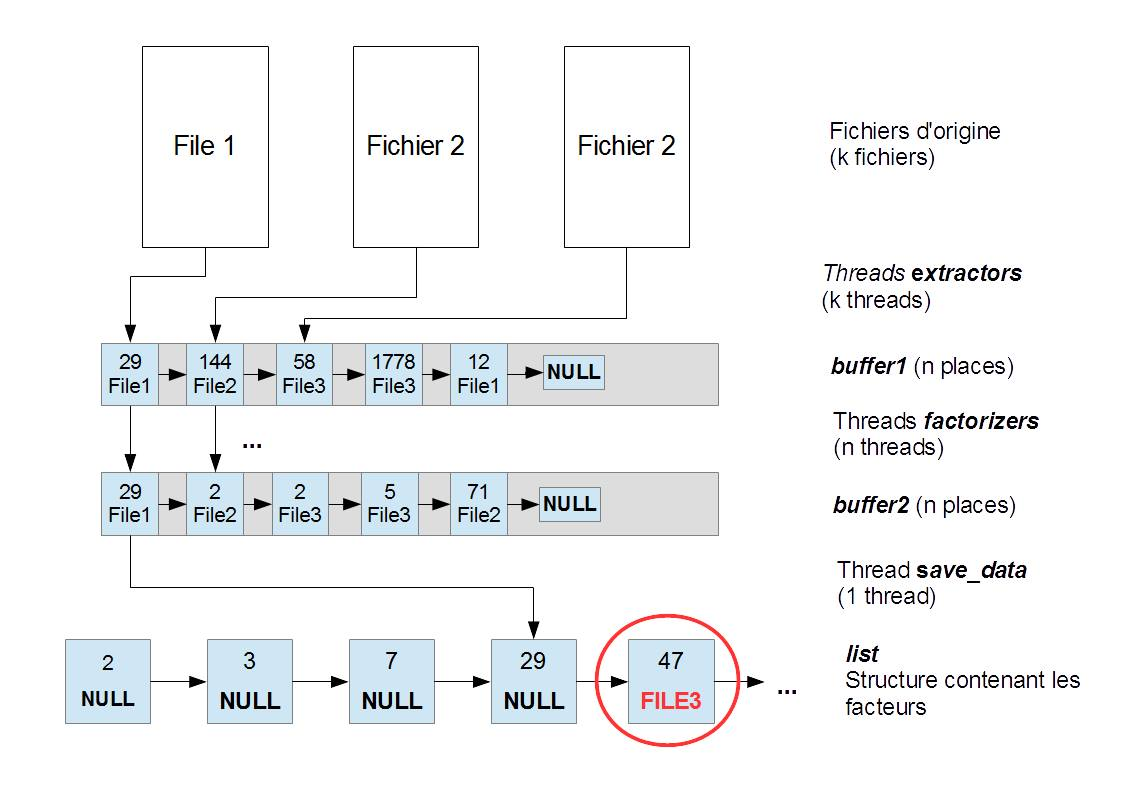
\includegraphics[scale=0.3]{img/arch.jpg}
	\caption{L'architecture de notre programme.}
	\label{fig:arch}
\end{figure}

\\
Comme dit précédemment, nous avons défini une structure permettant de représenter un nombre \emph{number} définie par son contenu \emph{n} (de type uint64\_t) et d'une chaîne de caractère \emph{origin} contenant le nom de son fichier d'origine.\\
Pour déterminer le facteur premier n'apparaissant qu'une seule fois dans la liste chaînée \emph{list}, nous avons procédé comme suit : lorsque une number est inséré dans la liste (ordonnée), on vérifie d'abord si un number possédant le même n ne s'y trouve pas déjà. Si ce n'est pas le cas, on se contente de l'insérer normalement, sinon, on change la variable origin du node en NULL. Ainsi, si un facteur n'apparaît qu'une seule fois, sa variable origin sera différente de NULL.\\
\\
Notre programme est divisé en plusieurs fichiers (vous trouverez parmi eux un README pour de plus amples détails). Le corps principal du programme se trouve dans upfact.c : c'est ce fichier qui sera compilé et exécuté. Dans core.c, nous avons mis l'ensemble des fonctions dépendantes des threads (l'extraction de fichiers, l'insertion dans la liste ainsi que la factorisation). L'algorithme de factorisation proprement dit se trouve quant à lui dans trial.c. D'autres fichiers plus modestes mais malgré tout importants sont aussi présents : perf.c contient la fonction relative à l'analyse de performances, io.c une fonction gérant diverses erreurs et stack.c les fonctions de gestion de la structure chaînée. Enfin, fopen.c contient les fonctions relatives à l'extraction de fichiers \emph{via} la librairie \emph{libcurl}. Ce fichier n'a pas été initialement écrit par nous mais est basé sur le code d'exemple conseillé dans les consignes de ce projet.\\
\\
Pour utiliser les threads à bon ascient, nous avons considéré la situation comme un problème de producteurs-consommateurs double. Les premiers producteurs sont les \emph{extractors} qui stockent les nombres dans le \emph{buffer1} qui sont consommés par les \emph{factorizers}. Ensuite, ces mêmes threads font office de producteurs du \emph{buffer2} où ils stockent les facteurs premiers consommés par le thread \emph{save\_data}. \\
Afin d'éviter les aléas du non-déterminisme, un tel problème doit être protégé comme suit : chaque buffer doit être protégé par un mutex (pour éviter les problèmes de section critique) et leur accès est réglé par deux sémaphores chacun : un pour leurs consommateurs, l'autre pour leurs producteurs.


\section{Performances}
Nous avons mesuré les performances de notre programme pour différents nombres
de threads de calculs et pour des fichiers contenant de très grands nombres.
Les résultats de ces mesures sont indiqués dans la figure \ref{fig:speedup}.
On constate que la figure \ref{fig:speedup} ressemble fortement à la loi d'Amdahl.

\paragraph{Remarque importante}
Comme expliqué dans la section précédente, pour permettre de mieux observer
les améliorations de performances en fonction du nombre de threads, nous avons
utilisé un algorithme de factorisation naïf. Celui-ci rend le programme assez
lent pour de très gros nombres (à titre d'exemple 2200 secondes pour 1 threads). 
\\
On constate une nette amélioration du temps d'exécution par rapport au nombre de threads jusqu'à environ 10 threads (figure 1). Par après, les performances s'améliorent toujours mais dans une moindre mesure. Ce résultat est également bien traduit par la figure 2, illustrant l'accélération du programme par rapport au nombre de threads. En définitive, ces résultats sont conformes à ceux escomtés et à la Loi de Amdahl : l'amélioration des performances est considérable jusqu'au seuil des threads physiques où elles s'atténuent.

\begin{figure}[ht]
	\centering
	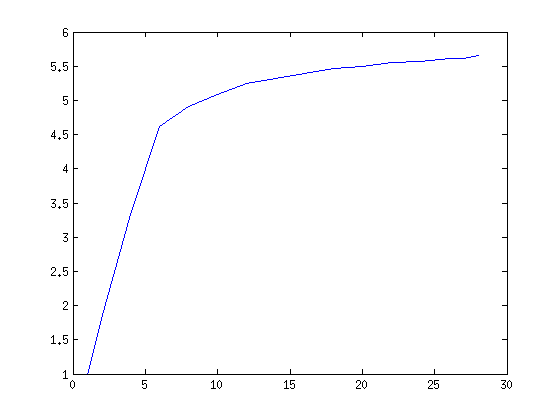
\includegraphics[scale=0.8]{img/speedup.png}
	\caption{Accélération du programme en fonction du nombre de threads sur un processeur i7 3770k (12 coeurs)
	avec 8GB de RAM.}
	\label{fig:speedup}
\end{figure}

\begin{figure}[ht]
	\centering
	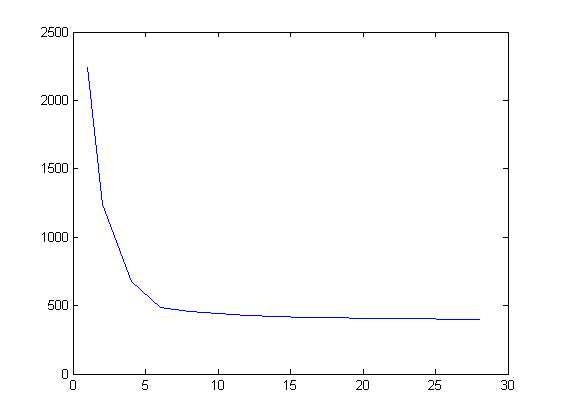
\includegraphics[scale=0.8]{img/time.png}
	\caption{Temps d'éxécution en fonction du nombre de threads sur un processeur i7 3770k (12 coeurs)
	avec 8GB de RAM.}
	\label{fig:time}
\end{figure}


\end{document}